\documentclass[11pt,letterpaper]{article}
\usepackage{fullpage}
\usepackage[pdftex]{graphicx}
\usepackage{amsfonts,eucal,amsbsy,amsopn,amsmath}
\usepackage{url}
\usepackage[sort&compress]{natbib}
\usepackage{natbibspacing}
\usepackage{latexsym}
\usepackage{wasysym} 
\usepackage{rotating}
\usepackage{fancyhdr}
\DeclareMathOperator*{\argmax}{argmax}
\DeclareMathOperator*{\argmin}{argmin}
\usepackage{sectsty}
\usepackage[dvipsnames,usenames]{color}
\usepackage{multicol}
\definecolor{orange}{rgb}{1,0.5,0}
\usepackage{multirow}
\usepackage{sidecap}
\usepackage{caption}
\renewcommand{\captionfont}{\small}
\setlength{\oddsidemargin}{-0.04cm}
\setlength{\textwidth}{16.59cm}
\setlength{\topmargin}{-0.04cm}
\setlength{\headheight}{0in}
\setlength{\headsep}{0in}
\setlength{\textheight}{22.94cm}
\allsectionsfont{\normalsize}
\newcommand{\ignore}[1]{}
\newenvironment{enumeratesquish}{\begin{list}{\addtocounter{enumi}{1}\arabic{enumi}.}{\setlength{\itemsep}{-0.25em}\setlength{\leftmargin}{1em}\addtolength{\leftmargin}{\labelsep}}}{\end{list}}
\newenvironment{itemizesquish}{\begin{list}{\setcounter{enumi}{0}\labelitemi}{\setlength{\itemsep}{-0.25em}\setlength{\labelwidth}{0.5em}\setlength{\leftmargin}{\labelwidth}\addtolength{\leftmargin}{\labelsep}}}{\end{list}}

\bibpunct{(}{)}{;}{a}{,}{,}
\newcommand{\nascomment}[1]{\textcolor{blue}{\textbf{[#1 --NAS]}}}


\pagestyle{fancy}
\lhead{}
\chead{}
\rhead{}
\lfoot{}
\cfoot{\thepage~of \pageref{lastpage}}
\rfoot{}
\renewcommand{\headrulewidth}{0pt}
\renewcommand{\footrulewidth}{0pt}


\title{11-712:  NLP Lab Report}
\author{Jonathan Barker}
\date{April 26, 2013}

\begin{document}
\maketitle
\begin{abstract}
This a report on the development of HindiMorph, an open source morphological analyzer for Hindi. Hindi is a morphologically rich language for which I have created an analyzer. I present a brief background on the language and the phenomena I hope to analyze. Existing work on and tools for Hindi morphology are then reviewed. After that I explain the system design and document my progress, results and ideas for future work. 
\end{abstract}

HindiMorph is an open source morphological analyzer for the Hindi language. Being a morphologically rich language, Hindi may be easier to work with when it's morphemes are tagged instead of just using the surface forms found in text. This report provides a brief introduction to the Hindi language and covers the morphological phenomina that HindiMorph hopes to analyze, in addition to summarizing previous work and other existing tools. It also documents the design of the system as well as it's development and performance.

\section{Basic Information about Hindi}
According to \cite{ethnologue}, Hindi (also Khadi Boli or Khari Boli) is an Indo-European language from India that is spoken by 181,676,620 people world-wide. It is the official language of India and derives much of its formal vocabulary from Sanskrit. \\
\\
Hindi is a fully developed language written in the Devanagari script. The script is written from left to right and is characterized by the long horizontal lines connecting the letters of each word. Devanagri uses spaces, making tokenization simpler.
\begin{figure}[h]
  \caption{An example of Devanagri script in a dictionary.}
  \centering
  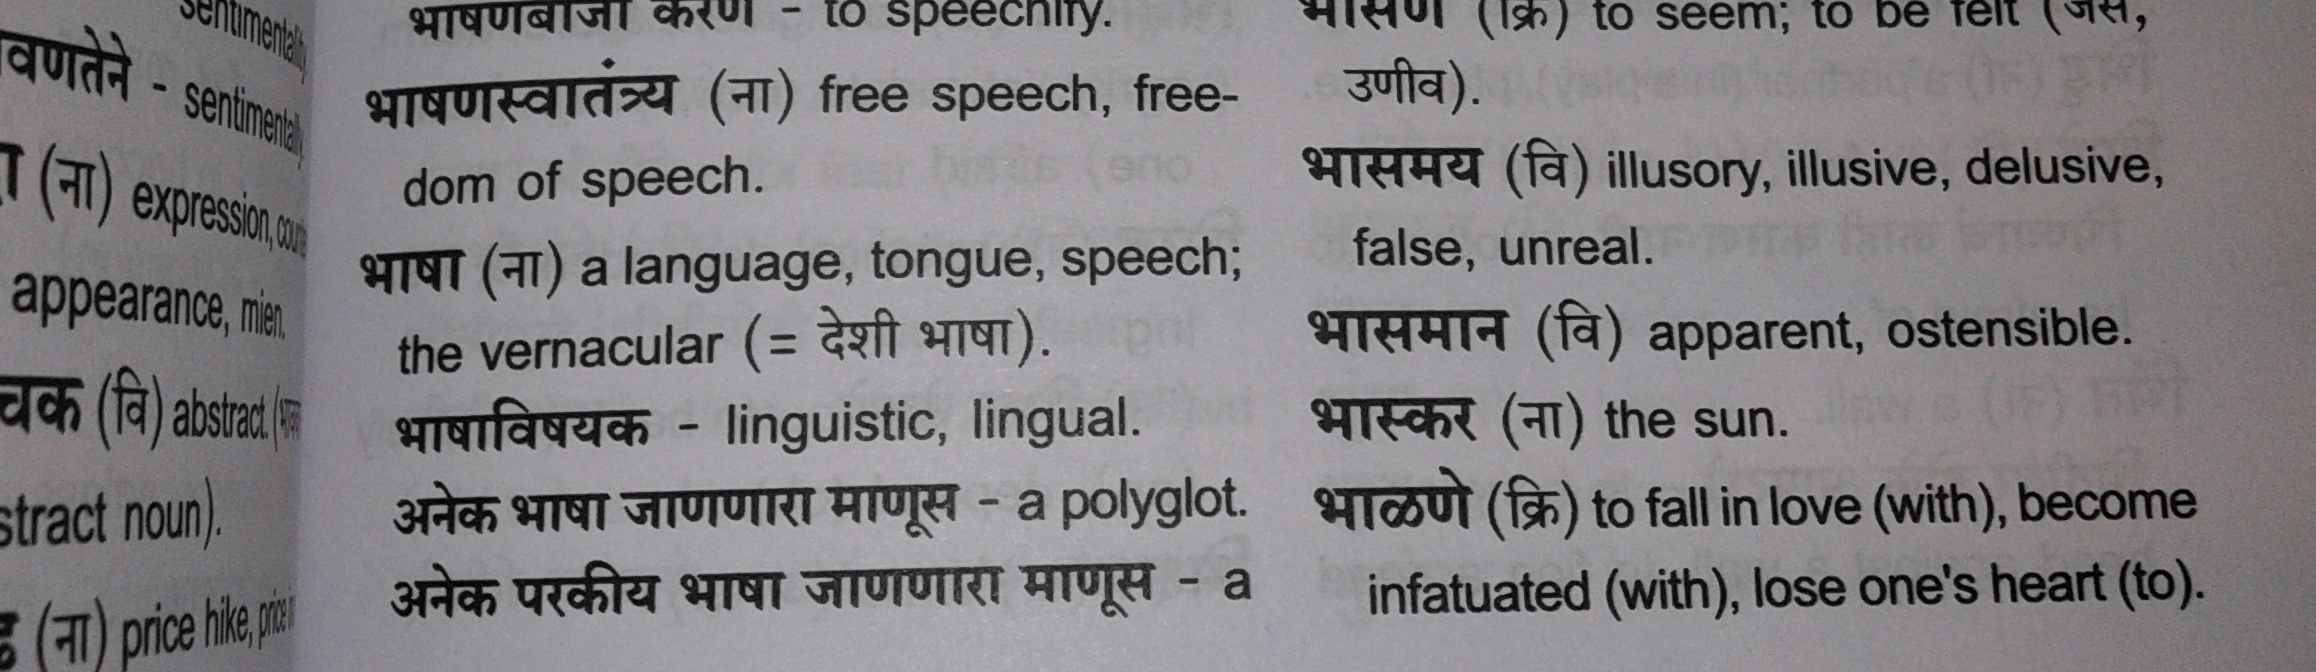
\includegraphics[scale=0.15]{devanagri.jpg}
  \label{script}
\end{figure}
The image in Figure~\ref{script} is an example of Devanagri in a dictionary. \\
\\
Hindi has an SOV grammar and a rich morphology. There are two genders, two numbers, and three cases (direct, oblique, and vocative) for nouns as well as two types of nouns (type-I and type-II) within these categories. Adjectives must agree with nouns in gender, case and number athough some do not decline at all. Verbs have 3 aspects, tense/mood and must agree in gender and number \cite{snell}. There are many declensions and conjugations in Hindi, making the development of a morhpological analyzer useful.
\section{Past Work on the Morphology of Hindi}
A seminal work on the grammar and morphology of Hindi is J.T. Platt's ``A grammar of the Hindustani or Urdu language'', written in 1873. In 1997 Rajendra Singh published ``Hindi morphology: a word-based description'', a work that intends to be a mostly comprehensive study of Hindi morphology. Reviewer Alan S. Kaye states that the book is less influential than Platt's and takes issue with a few details of the book. In addition to these, Shaligram Shukla's ``Hindi morphology'' is a good reference for information about Hindi morphology. Smriti Singh has published papers looking at Hindi's nominal and verbal morphology from the Distributed Morphology (DM). Together these resources offer a comprehensive view on the phenomena involved in Hindi morphology.\\
\\
On the system development side of things a few papers have been published concerning building morphological analyzers for Hindi. These papers provide insight on the results and difficulties of building a morphological analyzer for Hindi. They discuss issues surrounding tranlsiteration, visualization, ease of installation and use, morphological modeling (derivational vs. inflectional), and ambiguity (Kanuparthi et. al., 2012; Goyal et. al., 2008; Bögel et al. 2007). Focused on downstream applications like MT, these papers offer a pragmatic view of how to go about modeling Hindi morphology. \\
\section{Available Resources}

\nascomment{include discussion of your corpora}

\section{Survey of Phenomena in Hindi}

\section{Initial Design}

\section{System Analysis on Corpus A}

\section{Lessons Learned and Revised Design}

\section{System Analysis on Corpus B}

\section{Final Revisions}

\section{Future Work}





\bibliographystyle{plainnat}
\bibliography{refs}
\label{lastpage}
\end{document}
